\documentclass[jou]{apa} %can be jou (for journal), man (manuscript) or doc (document)
%
%
%these next packages extend the apa class to allow for including statistical and graphic commands
\usepackage{url}   %this allows us to cite URLs in the text
\usepackage{graphicx}  %allows for graphic to float when doing jou or doc style

% 11-07 is the FDG paper.
% 10-08 is robert's thesis.
% APA style info at: http://www.ilsp.gr/homepages/protopapas/apacls.html

% We need a table that shows "Dorm Energy Competition Design", with entries to say if the
% designers revealed (a) how baseline data was collected; (b) how the ranking was
% determined; (c) what factors were taken into account in creating the ranking; (d) was
% data collected after the competition to look for rebound effect; (e) was there evidence
% of short-term, unsustainable behavior change; 

% Proposal: let the teams create an argument for why they should win (this encourages more
% introspection and potentially data gathering.)

\title{Lights Off.  Game On? \\ \ 
       Myths and misperceptions in energy competition game design}
\author{Philip M. Johnson and Yongwen Xu and Robert S. Brewer}
\affiliation{Collaborative Software Development Laboratory \\ Information and Computer
  Sciences \\ University of Hawaii \\ Honolulu, HI USA \\ johnson@hawaii.edu}

\abstract{

  The Kukui Cup project investigates the use of ``meaningful play'' to facilitate energy
  awareness, conservation and behavioral change.  Each Kukui Cup Challenge combines real
  world and online environments in an attempt to combine information technology, game
  mechanics, educational pedagogy, and incentives in a synergistic and stimulating
  fashion.  We challenge players to: (1) acquire more sophistication about energy concepts
  and (2) experiment with new behaviors ranging from micro (such as turning off the lights
  or installing a CFL) to macro (such as taking energy-related courses, joining
  environmental groups, and political/social advocacy.)

  To inform the design of the inaugural 2011 Kukui Cup, we relied heavily on the design of
  prior collegiate energy competitions, of which there have been over 150 in the past few
  years.  Published accounts of these competitions indicate that they achieve dramatic
  reductions in energy usage (a median of 22\%) and cost savings of tens of thousands of
  dollars.  In our case, the data collected from the 2011 Kukui Cup was generally in
  agreement, with observed energy reductions of up to 16\% when using
  standard analysis techniques.  However, our analysis process caused us to look more
  closely at the methods employed to produce outcome data for energy competitions, with
  unexpected results.

  We now believe that energy competitions make significant unwarranted assumptions about
  the data they collect and the way they analyze it, which calls into question the
  accuracy of published results from this literature.  We believe a closer examination of
  these issues by the community can help improve the design not only of future energy
  challenges, but other similar forms of ``serious games for sustainability''.

  In this paper, we describe the Kukui Cup, the design myths and misperceptions it
  uncovered, and how we believe these issues should inform the design of future forms of
  ``meaningful play'' with respect to energy.

}


\acknowledgements{The Kukui Cup is supported in part by grant IIS-1017126 from the
  National Science Foundation, by the University of Hawaii (Facilities Management,
  Housing, and Information and Computer Sciences), and by the Hawaii State
  Department of Business, Economic Development, and Tourism.  We gratefully acknowledge
  the 418 players of the 2011 Kukui Cup and the members of the project team in addition to
  the authors who made the vision a reality: Kaveh Abhari, Hana Bowers, Greg Burgess,
  Caterina Desiato, Michelle Katchuck, Risa Khamsi, Alex Young, and Chris Zorn.}

\shorttitle{Myths and misperceptions in energy challenge game design}
%\rightheader{Right header}
%\leftheader{Left Header}

\begin{document}
\maketitle 

\section{Introduction}  

The rising cost, increasing scarcity, and environmental impact of fossil fuels as an
energy source makes a transition to cleaner, renewable energy sources an international
imperative.  One barrier to this transition is the relatively low cost of current
energy, which makes financial incentives less effective. Another barrier is the historical
success of electrical utilities in making energy ubiquitous, reliable, and easy to access,
thus enabling widespread ignorance about basic energy principles
and trade-offs.  In Hawaii, the need for transition is especially acute, as our state
leads the nation both in the price of energy and in reliance on fossil fuels as an energy
source.

Moving away from petroleum is a technological, political, and social paradigm shift,
requiring citizens to not only think differently, but behave differently with respect to
energy policies, methods of generation, and their own consumption. Unfortunately, there is
no tradition of teaching ``energy'' as a core subject area in the United States, even
though this subject appears to be one of the most important emergent issues of the 21st
century. Anecdotal reports indicate the lack of basic energy literacy at the secondary
school level \cite{Ammons2010}.

%% It would be nice to have more citations and examples regarding the "lack of basic energy literacy."

One of the most widespread and successful approaches to raising the profile of energy use
is the collegiate dorm energy competition, which has been held on over 150 campuses
in the past few years \cite{Hodge2010}.  Published documents report that these
competitions are extremely successful.  Hodge states median reductions in energy use of
22\% and a maximum reduction of 80\% for the competitions she studied. A case study of
Elon University claims that a seven week competition reduced energy consumption by
231,454 kWh and produced \$2,000 in electicity cost savings per week \cite{Durr2010}.

In an attempt to build upon these promising initial results, we began the Kukui Cup
project in 2010.  Our goal is to expand the scope from a relatively simple ``competition''
where the primary outcome measure is energy consumption in kilowatt-hours (kWh) to a more
elaborate ``challenge'' in which we combine information technology, community-based social
marketing, serious games, and educational pedagogy to support sustained change in
sustainability-related behaviors.  In addition to measuring kWh consumption, the Kukui Cup
also implements a point system intended to measure player involvement with educational
materials, workshops, excursions, and group engagement.  Through a series of challenges
held in residence halls at the University of Hawaii and elsewhere, we are gaining
deeper insight into how these various factors contribute to positive behavioral change.

Our first Kukui Cup challenge was held at the University of Hawaii in Fall, 2011 for the
1,000 students in the Hale Aloha residence halls. The challenge divided the students into
20 teams (called ``lounges'') of approximately 50 students each.  We started measuring
energy consumption for most teams at three weeks prior to the competition, although
several teams did not have operational energy meters until shortly before the competition
started. We followed the traditional approach of using this data to produce baselines as a
way of assessing whether and to what extent energy reductions occurred as a result of the
challenge.

Our initial analyses of the data we collected during the challenge appeared promising.
Over 400 of the students participated in the three week challenge, spending over 850 hours
in the online environment.  Student feedback regarding both real world and online aspects
of the challenge was uniformly positive.  Some teams appeared to achieve a 10-16\%
reduction in their energy usage during the challenge.  Participating students made over
1,000 commitments and earned over 80,000 points.

As we continued to look at the outcomes from the 2011 challenge in order to understand
how to better support sustainable behavioral change, we began to be troubled by the way
we and other dorm energy competitions measure outcomes, and the variety of unwarranted
assumptions underlying the measurements and results.  These design problems
are not merely theoretical or scientific: they have a direct impact on the experience of
participants and the effectiveness of these competitions as ``meaningful play''.  For
example, the baseline calculation method used during the 2010 Campus Conservation
Nationals energy competition led some students at Oberlin College to stop participating in
the competition ``out of frustration'' \cite{Willens2010}.

Making matters worse, published reports concerning energy competitions rarely document
how, for example, baseline energy consumption is calculated, or what happens to energy
consumption after the competition ends.  Without information like this, it is hard to
assess the true ``meaningfulness'' of the ``play''.  For example, if baseline-based
measurement of energy reduction enables a team to ``coast to victory'' with minimal
behavior change, is the play ``fair''? If energy consumption returns immediately to
pre-competition levels after the competition ends, then was the play ``meaningful'', no
matter what the level of reduction was achieved during the competition?

This paper presents our findings to date about how to better understand the impact of
energy competitions and challenges as meaningful play, and how to improve this impact over
time.  We believe this process must start with a better understanding of the limitations
of {\em kWh consumed} as an outcome measure, as tempting a metric as it might be.  We
argue that ``behavior'' must be interpreted and measured more broadly and that games must
be designed to promote and reward a much more diverse spectrum of behavior change.  Rather
than reward students for unsustainable changes such as unplugging vending machines (as at
Oberlin College \cite{Petersen07a}) or camping outside during the competition (as at
Carleton College \cite{Hodge2010}), future games could reward students for sustainable
changes such as enrolling in a class on energy in an upcoming semester, or joining an
environmental group that promotes renewable energy.

The next section of this paper provides a brief overview of the Kukui Cup.  The following
section presents the myths and misperceptions that we believe to be widespread in the
design and reporting of current energy competitions. We conclude with our recommendations
for how we and others should design future energy challenges to be more effective as
meaningful play.

\section{The Kukui Cup}

A defining feature of Kukui Cup challenges is a blend of real world and virtual world
activities, all tied together through game mechanics.  In the real world, players
participate in workshops and excursions, win 
prizes, and most importantly, learn about their current lifestyle and its impact on
energy consumption.  In the online world of the Kukui Cup web application, players
earn points, achieve badges, increase their sustainability "literacy" through readings and
videos, and use social networking mechanisms to engage with friends and family about the
issues raised. The challenge is designed to make real world and online activities
complementary and synergistic.

Each Kukui Cup Challenge is typically designed with the following goals for its participants:
\begin{itemize}
\item Increase {\bf knowledge} about energy issues;
\item Gain {\bf insight} about the impact of one's current behaviors and how to change
  them for more effective energy usage;
\item Build {\bf community}, through awareness of local and national sustainability organizations and initiatives;
\item Create {\bf commitment}, from minor (turn off the lights when not in use) to major (pursue a profession related to sustainability).
\end{itemize}

To create sophisticated games based upon energy consumption, it is helpful to
collect real-time energy data from meters, store the data, perform analyses on the data, and
visualize the results. We developed WattDepot \cite{csdl2-10-05} to provide an open source, vendor-neutral
framework for energy data collection, storage, analysis, and visualization.  WattDepot is
useful not only as technology infrastructure for the Kukui Cup, but as infrastructure for
other energy-related initiative such as the Smart Grid.

Implementation of game mechanics is provided by another system we developed called
Makahiki \cite{csdl2-11-07}.  It provides an open source, component-based, extensible environment for
developing sustainability challenges such as the Kukui Cup and tailoring them to the needs
of different organizations.  One configures the Makahiki framework to produce a "challenge
instance" with a specific set of game mechanics, user interface features, and experimental
goals.  Makahiki provides sophisticated instrumentation to support evaluation of how well
the game mechanics supported the organization's goals for the challenge. 




\section{Myths and misperceptions in energy challenge game design}

The preceding section presented the design and implementation of the 2011 Kukui Cup along
with some basic outcome data in a manner consistent with the way many other energy
competitions have been presented.  Perhaps the most significant outcome from the 2011
Kukui Cup was the insight that virtually all energy challenges, when viewed as game
designs, could have a variety of fundamental flaws: they might not create a fair game,
they might not measure what they think they are measuring, they might not measure the
right things, and they might not achieve the right outcomes.  In this section we discuss
how we came to these realizations.

To begin: a fundamental property of energy challenges is competition, and a fundamental
property of competitions is the ability to creating rankings.  The first set of myths
concern the flaws related to competition and ranking.


\subsection{Myth \#1: Percentage reduction from baseline is a valid ranking method}

In general, there are two methods for creating rankings in energy competitions: (1) by total
energy consumption or (2) by reduction from a baseline.

The first ranking method is simple: order the teams according to their total energy
consumption (from least to most) during the competition interval.  As illustrated in Table
\ref{table:total-reduction}, if Team A consumes 1,140 kWh during the competition period,
and Team B consumes 1,239 kWh, then Team A wins.  This is the simplest method, but
produces a valid ranking only if every team is equivalent with respect to the factors
affecting their energy consumption.  For example, to use this ranking method, every team
should have the same number of members.  If Team A has 50 members and Team B has 60
members, then Team A's victory is due to an unfair advantage.  In addition, every team
should have the same energy infrastructure.  If, for example, Team A lives in a
well-insulated building and Team B lives in a poorly insulated building, then Team A again
wins due to an unfair advantage.  Because it is so difficult to obtain equality
among teams with respect to all significant energy consumption factors, and because the unfairness of
a competition using this ranking method can be so obvious, this method is relatively
uncommon.

\begin{table}[tbp]
\caption{Total energy reduction ranking method. Winning number in bold.}
\label{table:total-reduction}
\begin{tabular}{p{0.5in}p{0.5in}}\thickline
Team  & Actual (kWh) \\ \hline
A     & {\bf 1,140}        \\  
B     & 1,239        \\ \hline
\end{tabular}
\end{table}


To address the obvious inequities with using total energy consumption second, the more
common method is to compute a ``baseline'' for each team based upon
historical usage and produce rankings for teams based upon reductions from this baseline.
The goal is to normalize energy consumption so that teams with differing factors affecting
their energy consumption can be fairly ranked. Table \ref{table:percentage-reduction}
illustrates approach.

\begin{table}[tbp]
\caption{Reduction from baseline ranking method. Winning numbers in bold.}
\label{table:percentage-reduction}
\begin{tabular}{p{0.5in}p{0.5in}p{0.5in}p{0.5in}p{0.5in}}\thickline
Team  & Baseline (kWh) & Actual (kWh) & Reduction (kWh) & Percent Reduction  \\ \hline
A     & 1,200          & 1,140        & 60                 & {\bf 5 \%}              \\  
B     & 1,300          & 1,239        & {\bf 61}                 & 4.6 \%            \\ \hline
\end{tabular}
\end{table}

As in the prior example, Team A consumes 1,140 kWh and Team B consumes 1,239 kWh.  Using
energy data collected prior to the competition, a baseline of 1,200 kWh was established
for Team A and a baseline of 1,300 kWh was established for Team B.  

What is interesting about this example is that there are two winning numbers. Team A wins
if percentage reduction from baseline is used as the ranking method, while Team B wins if
absolute reduction from baseline is used as the ranking method.  In all of the energy
competitions we have seen, it is percentage reduction from baseline, not absolute
reduction from baseline, that used as the ranking method.

The uniform use of percentage reduction from baseline for ranking exposes the first
problem with the use of baselines, because there is no {\em a priori} reason that
percentage reduction from the baseline produces a more fair ranking than absolute
reduction from the baseline.  To see why this is so, consider the following 
scenario where Team A lives on one floor and Team B lives on an adjacent floor.  The two
floors are similar in structure and occupancy except that Team B's floor includes a shared
laundry room.  In this case, the most fair way to produce a ranking is to calculate the
energy consumption of the shared laundry room, subtract that consumption from Team B's
data, then use absolute values to rank the floors.  Put simply, the two teams should be
considered equal once the load from the shared laundry room is factored out.

\begin{table}[tbp]
\caption{Adjusted absolute consumption ranking method. Winning numbers in bold.}
\label{table:adjusted-absolute-reduction}
\begin{tabular}{p{0.5in}p{0.5in}p{0.5in}p{0.5in}p{0.5in}}\thickline
Team  & Baseline (kWh) & Actual (kWh) & Adjusted (kWh) & Percent Reduction  \\ \hline
A     & 1,000          & 900          & 900            & {\bf 10 \%}        \\  
B     & 1,300          & 1,180        & {\bf 880}      & 9 \%               \\ \hline
\end{tabular}
\end{table}

Table \ref{table:adjusted-absolute-reduction} illustrates this scenario.  Team A reduces
their consumption by 100 kWh from the baseline, for a winning percentage reduction of 10\%. Team B
reduces their consumption by 120 kWh from the baseline, for losing percentage reduction of
9\%.  But the fairer way to compare these two teams is to simply subtract out the 300 kWh
of energy consumed by the laundry room, then compare the two consumptions directly.  Under
this ``adjusted'' ranking scheme, Team B wins because their adjusted consumption of 880
kWh is less than Team A's consumption of 900 kWh.

Of course, adjusted absolute consumption is not a panacea.  If Team A has 50 players and
Team B has 70 players, then some sort of percentage-based normalization to create a ``per
capita'' consumption is required to provide a fair ranking.  In many cases, some
combination of absolute adjustment (to compensate for structural differences like laundry
rooms) and percentage-based adjustment (to compensate for differences in number of
players) might be required.

Our conclusion is the following: to produce a valid ranking based upon energy consumption,
you must not only successfully measure ``normal'' energy consumption, you must also
determine the reasons behind the differences measured, because those reasons are crucial
to creating a fair ranking.

\subsection{Myth \#2: Representative energy data can be collected immediately prior to the competition}

The preceding section assumes that representative, or ``normal'' energy usage can be
determined and used as a baseline, and then exposes the problems that arise in using such
data to create a valid ranking.  Let's now step back and consider the question: is it
possible to gather energy data immediately prior to the competition and be confident that
it reflects ``normal'' usage during the competition?

Many energy competitions create baselines using the average energy consumption from
several weeks immediately prior to the start of competition.  Using recent data has two
significant advantages. First, baseline data is based upon the energy usage of the players
actually engaged in the competition.  Second, baseline data is based upon the state of the
infrastructure (buildings, appliances, etc.) as it will be during the competition.

The problem is that after seeing real data, it becomes much less obvious how to use it to
predict ``normal'' conditions during the competition.  For example, Figure
\ref{fig:kukuicup-baseline-data-chart} shows data from the three weeks prior to the
Kukui Cup 2011 energy challenge for five of the 20 teams.

\begin{figure*}[htbp]
\begin{center}
\includegraphics[width=0.8\textwidth]{kc-baselines.2.eps}
\caption{Energy data for five teams for the weeks immediately preceding the 2011 Kukui Cup}
\label{fig:kukuicup-baseline-data-chart}
\end{center}
\end{figure*}

% Would be better for Y axis to be in kWh and Y axis scale from 600 kWh to 1300 kWh (so
% variations are more visually apparent).  

What makes this data problematic for predicting ``normal'' conditions during the
competition are the variety of trends that can be observed in the different teams.  The
energy consumption of Mokihana-A, Mokihana-B, and Mokihana-D is trending upwards, while
the energy consumption of Mokihana-C and Mokihana-E is trending downwards.  The change can
be substantial: in the case of Mokihana-A, weekly energy consumption varied by approximately 30\% 
during the five weeks prior to the start of the challenge.

If we are to use this data to predict ``normal'' conditions during the challenge, we must
decide whether the trends represent persistent or transitory changes in consumption.  If we
believe the trends represent persistent changes, then the most appropriate choice is to
use the data immediately prior to the start of the challenge.  Under this assumption,
Mokihana-E would compete based upon a baseline consumption of approximately 1300 kWh.  

If, on the other hand, we believe the trends represent transitory changes in consumption,
then a better choice is to compute the baseline from the average energy usage over several
weeks prior to the competition.  Under this assumption, Mokihana-E would compete based
upon a baseline consumption of approximately 1100 kWh.  Thus, the choice of assumption
between persistent and transitory can make a difference of 15-20\% in the baseline value
in real world conditions.

All energy competitions that we have reviewed and that have published their baseline
calculation method use the averaging method, which implicitly assumes that observed trends
are transitory, not persistent.  But there is no {\em a priori} reason to assume that the
trends are transitory.  For example, perhaps a half dozen additional residents moved in to
Mokihana-E in late September, creating a persistent increase in energy consumption.  Using
data from early September to compute their baseline unfairly penalizes Mokihana-E by
producing a low baseline value that does not reflect normal conditions during October.

This same problem can occur when seasonal change is taken into account: the amount of
energy required to heat a team's residence might be significantly less in the month
preceding the competition if the competition is held in the Fall. Similarly,
heating-related energy consumption might be significantly more in the weeks preceding the
competition if the competition is held in the Spring.  This is another scenario in which
baseline data does not reflect normal conditions during the time period of the competition.

Seasonal change is not a theoretical issue: it created a significant problem with the
first Campus Conservation Nationals event \cite{Willens2010}.  According to John Peterson,
the ``baseline period... was, in some cases, resulting in percentage changes for
individual buildings... that were more attributable to changes in weather and other
factors than to the choices that students were making in their dorms.''

Our conclusion is the following:  Use of data collected immediately prior to the
competition can predict ``normal'' conditions during the competition with limited
accuracy. Our data indicates that baseline margin of error can reach 20\% under real
world conditions.

\subsection{Myth \#3: Representative energy data can be collected from years  prior to the competition.}

Given the problems with obtaining representative data immediately prior to the competition
for the purpose of creating baselines, an alternative is to use data from prior years.
This was in fact the choice made during the first Campus Conservation Nationals event
\cite{Willens2010}, as it was felt that such data would take into account seasonal changes
more effectively than data collected immediately prior to the competition. Unfortunately,
using data from prior years has significant validity problems when used to represent
``normal'' energy consumption during a future year, including:

\begin{itemize}

\item The residents of the building are typically different from year to year.
  Individuals can vary significantly in their energy consumption, and there is no {\em a
    priori} reason to believe that these differences simply average out. 

\item Building infrastructure can change from year to year. HVAC and other energy systems
  can degrade (leading to more energy consumption in future years) or be updated (leading
  to significantly less energy consumption in future years).  Similarly, building
  maintenance (such as weather stripping, lighting upgrades, etc.) can all change the
  energy consumption needs significantly.

\item Weather can vary considerably from year to year.  The number of heating degree days and cooling
  degree days in a given month can change considerably from one year to the next, leading
  to volatility in energy demand. 

\end{itemize}

As a concrete example, we examined the energy consumption data for the month of October
for the past 12 years in the Hale Aloha residence halls, and discovered variability of
over 30\% from one year to the next.

Our conclusion is the following: Similar to data collected immediately prior to a
competition, data collected from prior years can predict ``normal'' conditions during the
competition with only limited accuracy.  Our data suggests that the margin of error can easily
exceed 20\%.


\subsection{Myth \#4: Competition data can be used to estimate actual savings}

So far, we have called into question two important assumptions: (1) It is possible to
create a fair ranking system for teams in an energy competition; and (2) It is possible to
gather energy data that can serve as ``representative'' of the consumption to be expected
during the competition.  In this second case, we believe that the calculated
representative (or baseline) consumption can deviate by at least 20\% from the ``real''
value.

Unfortunately, if it is not possible to generate representative consumption with any
accuracy, then it is not possible to estimate actual savings with any accuracy.  This is
because estimated savings are always calculated by assuming that the baseline data not
only puts teams on an equal footing with each other for the purposes of the competition,
but also represents an accurate prediction of what each team would have consumed during
the time interval of the competition, had the competition not taken place.  

It is interesting to note that these two applications of baseline data are
independent: it is plausible to design baselines that succeed in creating a
level playing field among teams but that do not predict what the energy
consumption would have been in the absence of the competition.

Our conclusion is the following: virtually all published claims for dollar savings due to
energy competitions could not withstand a detailed analysis of the assumptions upon which
these claims were made.  As one example among many, we question the claim made by
the Campus Conservation Nationals that ``savings nationwide totaled 509,000 kilowatt
hours, \$50,200, and 816,00 pounds of carbon dioxide" \cite{Willens2010}.

\subsection{Myth \#5: The good guys win}

One intuitive assumption concerning energy competitions is that the winners will be those
who are most energy conscious.  In reality, under typical competition conditions
(i.e. collection of baseline data immediately prior to the competition, and the use of
percentage reduction from baseline for ranking), those teams who are most energy conscious
prior to the competition are at a distinct disadvantage.

This is because energy conscious teams are more likely to have already practicing 
conservation oriented behaviors prior to the competition period, and thus
their baseline energy use will be lower than their ``energy hog'' peers.  This makes it
harder for them to compete on the basis of percentage reduction, since they have ``less
fat'' from an energy perspective to cut from their consumption.  As a concrete example, we
discovered that it is not uncommon for residence hall rooms to have two refrigerators and
a few even had three refrigerators. For those residents, simply turning off one
refrigerator for the duration of the competition can achieve significant reductions in
consumption, whereas more ecologically conscious residents who chose to use only one
refrigerator would have to forego the refrigerator entirely to obtain the same reduction.

Note that it is not necessarily a flaw in competition design to have the ``bad guys''
win.  It is possible that giving positive reinforcement to that group of students might be
more effective than rewarding those who have already bought into energy conservation
principles. 


\subsection{Myth \#6: Competitions encourage sustainable change}

It is trivial to get a "perfect" 100\% reduction in energy; just flip the breaker.
Behaviors like unplugging vending machines are exactly similar.


\subsection{Myth \#7: Energy challenges measure the right thing}

Focusing on in-competition energy consumption is not meaningful.  Instead, to understand
the true value of energy competitions, one should instead measure: (1) post-competition
energy consumption; changes in participant knowledge as a result of competition; changes
in participant behavior (interpreted broadly: not just micro-behaviors like turning off
the lights but macro-behaviors such as choice of major)

Like looking under the lightpost for keys.

\section{Supporting more meaningful play through improved energy challenge game design}

Does all of this concern with accuracy and fairness really matter?  We claim it does, for
two reasons.  First, the fundamental goal of energy competitions is to increase the
literacy and sophistication of its participants.  Basing the competition on faulty data or
methods is, essentially, bad science, and we should be committed to providing players with
scientifically sound game design as a matter of educational principle.  Second, unfair
game design is tremendously demoralizing.  For example, an Oberlin student complained
about the unfair use of baselines and rankings in the Campus Conservation Nationals as
follows: ``We've turned off every [expletive] light in this building, dude, and it's not making
an [expletive] difference.''

Move away from ``competition'' and toward ``challenge''.

Change incentive and reward structure to depend less on pure kWh values, which are easy to
measure but not necessarily indicative of change, and toward broader definitions of
``behaviors''.

Change game mechanics so that short term, unsustainable changes in consumption are not
rewarded or incentivized (turn off every light in the building, etc.)   Teaching students
how to find the main circuit breaker and turn it off is not an interesting. 


\section{Reference materials}

\begin{itemize}

\item ``In the classroom, a lack of energy education'':
\url{http://www.indyweek.com/indyweek/in-the-classroom-a-lack-of-energy-education/Content?oid=1547796}.
Provides anecdotal evidence that students have very minimal energy literacy.

\item Chelsea Hodge (see dropbox folder kukucuip-2011/articles for slides).  Talks about a
  ``core component'' of a dorm energy competition being a ``short time frame'', which
  encourages students to ``go all out'', and provides as an example some Carleton College
  stduents who are camping out for a week to save energy.  This is clearly unsustainable
  behavior change. She talks about median reductions of 22\% and biggest reduction being
  80\%.  How did that number occur?

\item SLO residence hall competition.
\url{http://www.slideshare.net/AllianceToSaveEnergy/energy-and-water-residence-hall-competition}
No information on how baselines were calculated. 

\item CCN, Robert finds that 10\% reduction at stanford happened during finals week.
\url{https://groups.google.com/forum/?hl=en#!searchin/kukuicup/campus$20conservation/kukuicup/dYy6e0ORFE0/BxweJIznXRoJ}

\item More about baselines and relatively arbitrary changes.
\url{http://www.oberlinreview.org/article/dorm-energy-resource-competition-succeeds-despite/}.
A student told him, “We’ve turned off every fucking light in this building, dude, and it’s
not making a goddamn difference.” The baseline problem “killed us,” Sabo added.  Also, "Savings nationwide totaled 509,000 kilowatt hours, \$50,200, and 816,00 pounds of carbon dioxide."

Also: 
\url{https://oncampus.oberlin.edu/source/articles/2010/12/03/resource-reduction-competition-results}.
This talks about how bad choice of baselines made the competition less fair, also how
environmentally conscious students at Oberlin who have been conserving for years are
penalized because based upon percentage reduction. 

\item From Oberlin Review, ``To address the baseline problem, LDG will use “weather
  normalization,” a process that derives a baseline from five years of measurements,
  sidestepping problems of climate difference and inconsistent weather.''  But that now
  means building renovations etc. will not be controlled for.

\item From Green Cup at Berkeley, 
\url{http://tgif.berkeley.edu/index.php/grants/projects/2011-projects/28-greek-energy-savings}, 
results are always skewed towards winners, but 1/3 of the participants increased resource
usage during competition (some dramatically: 71\% increase in natural gas consumption).
Results are not looked at in depth to understand what exactly happened and why some places
increased in energy percentage-wise just as much as the top decreasers.

\item According to data compiled by Chelsea Hodges, over 150 colleges have had energy
  challenges in the 2010-2011 school year.  


\end{itemize}
\bibliography{sustainability,csdl-trs,smartconsumer,gamification,12-08}

\end{document}



